\chapter{Materiais e Métodos}
\label{cap:matmet}

Este capítulo descreve a área de estudo, as bases de dados utilizadas, o tratamento das informações, as medidas de autocorrelação espacial, a estatística de varredura espacial e a comparação entre as formulações, além dos recursos computacionais empregados e das definições descritivas adotadas.

\section{Área de Estudo}

O Brasil é o maior país da América do Sul em extensão territorial, com mais de 8,5 milhões de $km^2$, e possui população superior a 203 milhões de habitantes, segundo o último Censo Demográfico do Instituto Brasileiro de Geografia e Estatística (IBGE) \cite{ibge2022censo}. O território nacional está dividido administrativamente em 5.571 unidades territoriais\footnote{A divisão oficial vigente compreende 5.569 municípios, 1 Distrito Federal e 1 distrito estadual, totalizando 5.571 unidades. A malha de referência deste estudo baseia-se no Censo Demográfico de 2010, com 5.565 unidades; após a exclusão do distrito de Fernando de Noronha, o painel analisado contém 5.564 municípios, contando Brasília (DF) como município para a análise espacial.}, agrupadas em cinco grandes regiões: Norte, Nordeste, Centro-Oeste, Sudeste e Sul, como ilustrado na Figura~\ref{fig:mapa_regioes}. A Região Sudeste concentra a maior parte da população brasileira e responde por parcela substancial da atividade econômica nacional \cite{ibge2022atlas}.

Os biomas do país incluem Amazônia, Cerrado, Caatinga, Mata Atlântica, Pantanal e Pampa, distribuídos de forma heterogênea pelo território. O grau de urbanização é elevado, com grande parte da população em áreas urbanas. Densidade populacional, ocupação do território e condições de infraestrutura variam de forma expressiva entre municípios e regiões \cite{ibge2022atlas}.

\begin{figure}[H]
    \centering
    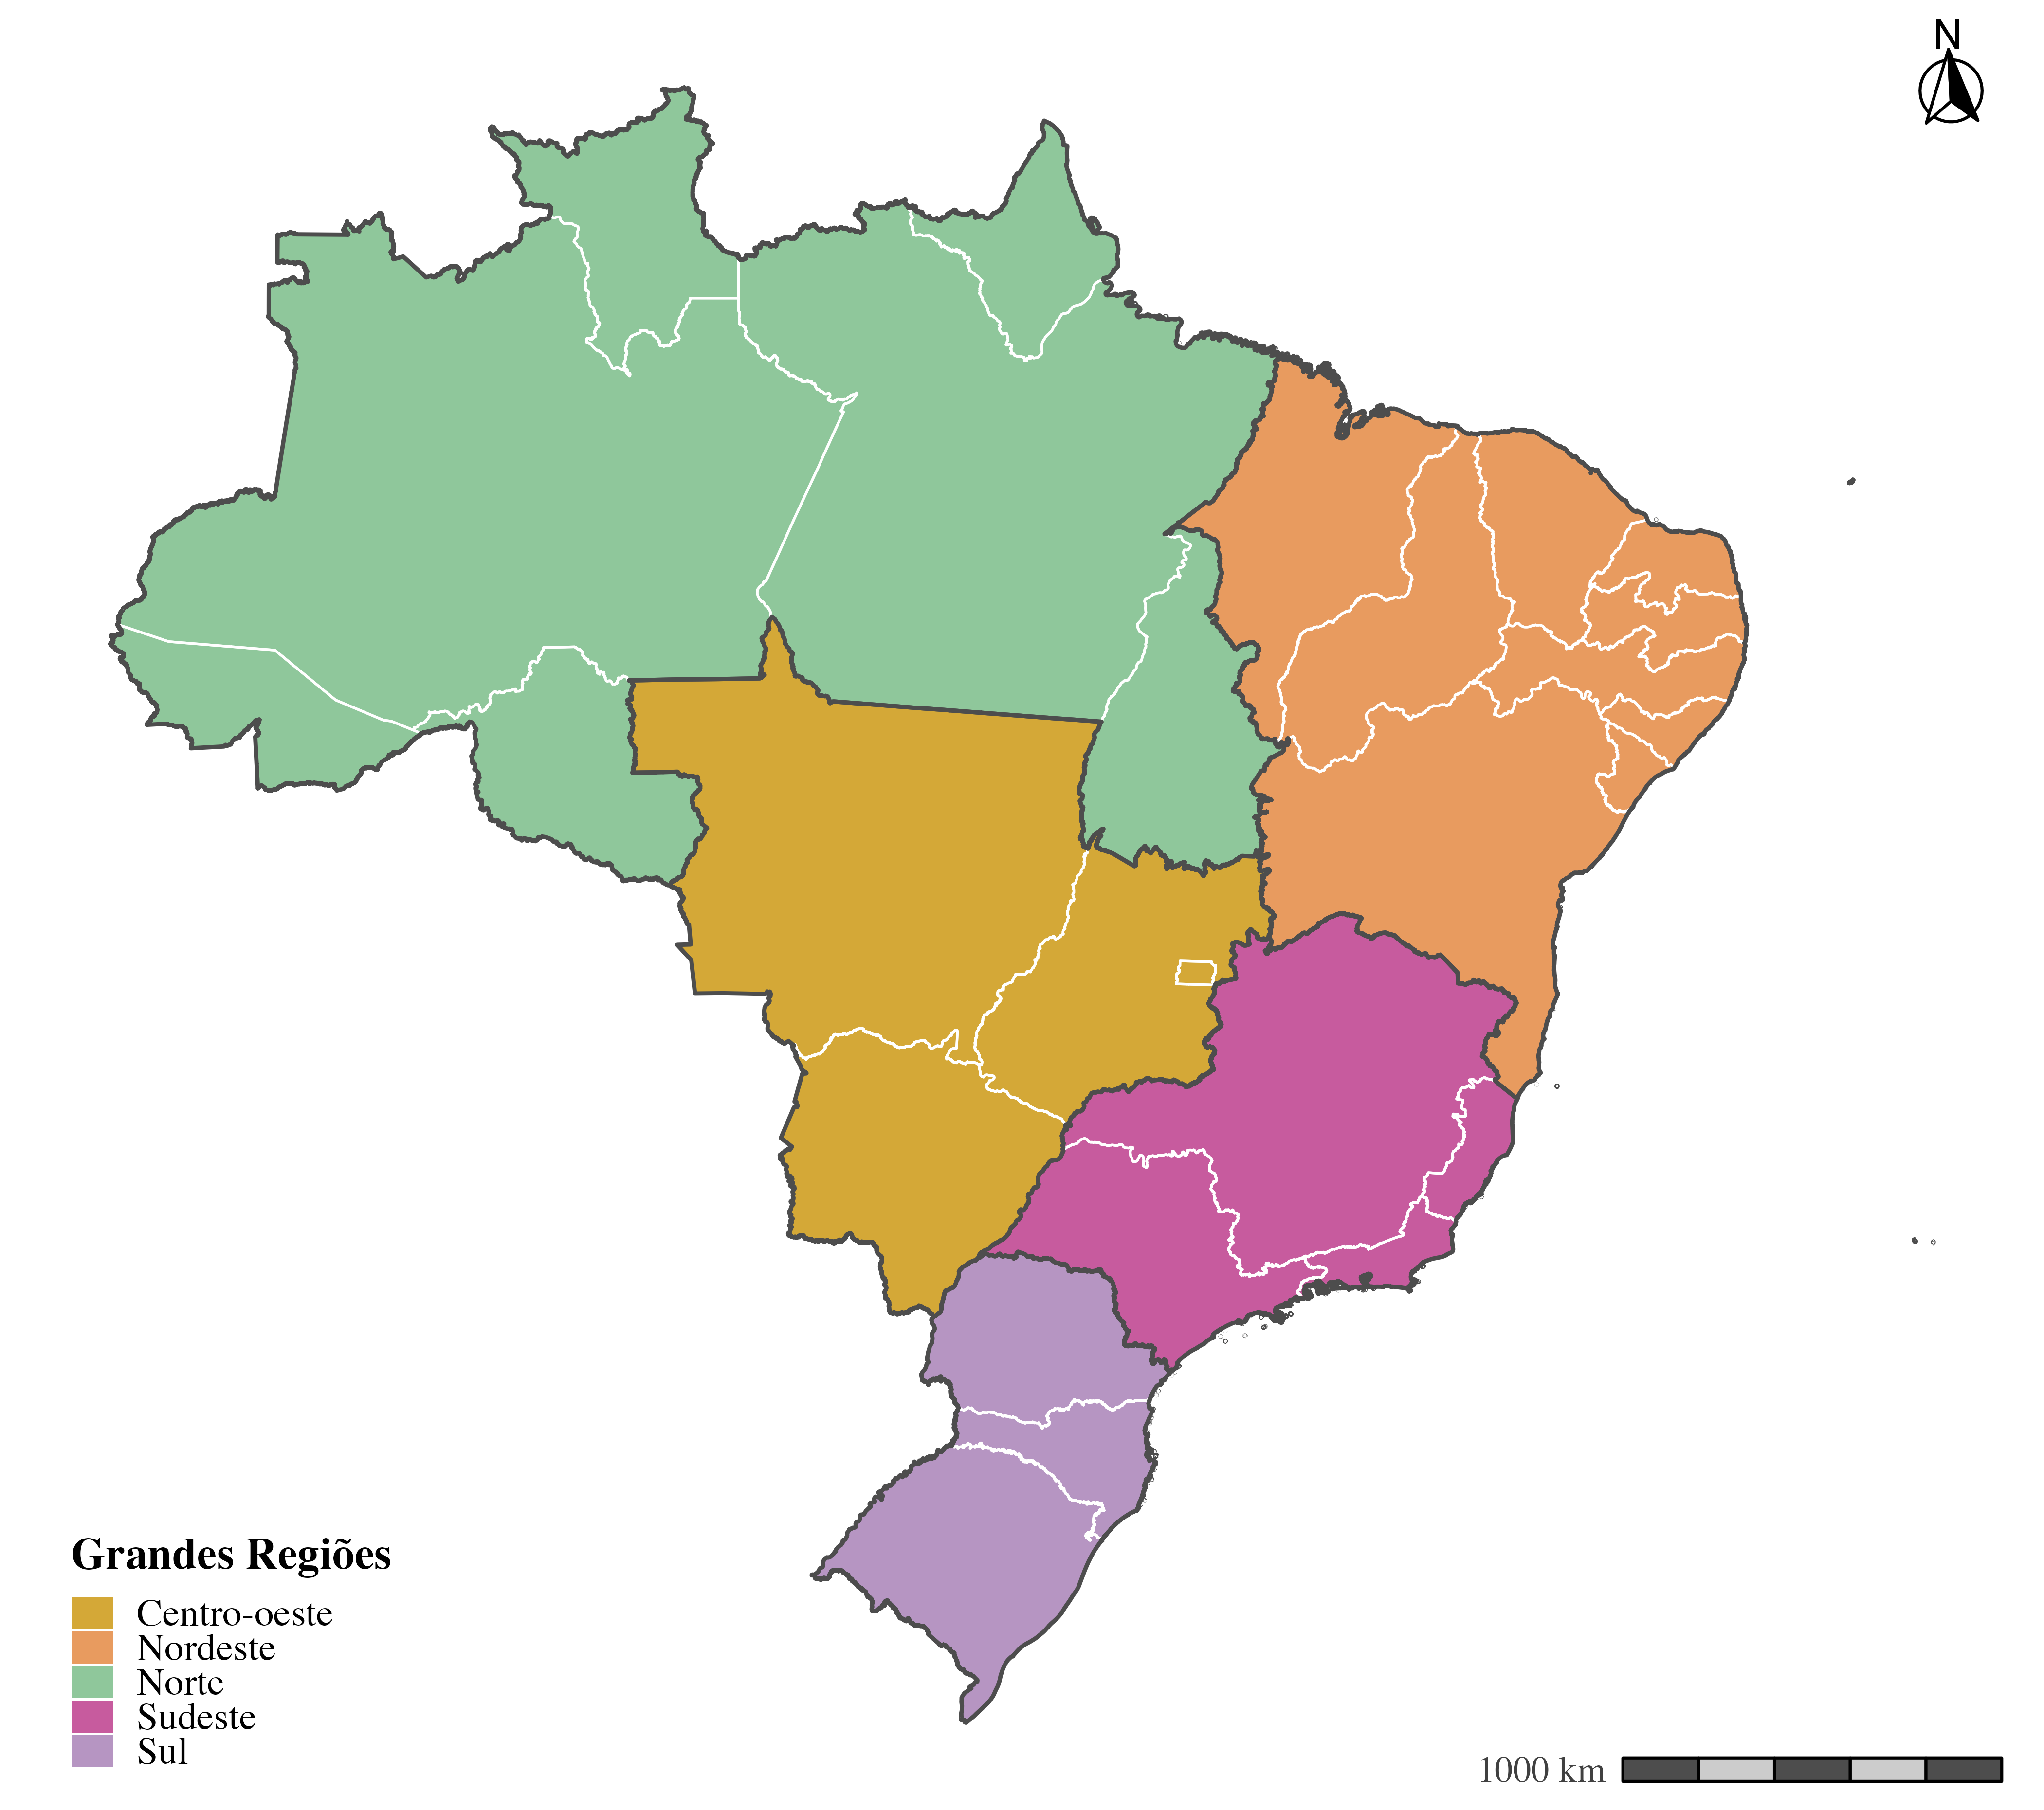
\includegraphics[width=0.76\textwidth]{fig_mapa_grandes_regioes.png}
    \caption{Divisão do território brasileiro por Grande Região. Fonte: IBGE.}
\label{fig:mapa_regioes}
    \vspace{0.3em}
    {\footnotesize\noindent\textit{Nota:} Divisão regional do IBGE; a malha municipal de análise segue a referência espacial de 2010.\par}
\end{figure}

\noindent \textbf{Grandes Regiões}

As características demográficas, territoriais e climáticas das grandes regiões vêm do Censo Demográfico 2022 \cite{ibge2022censo}, do Atlas Nacional do Brasil Milton Santos \cite{ibge2022atlas} e do Mapa de Clima do Brasil \cite{ibge2002clima}.

No Norte vivem aproximadamente 17,4 milhões de habitantes, com a menor densidade demográfica do país. Predomina a Floresta Amazônica, com grandes distâncias entre os principais centros urbanos. O clima é equatorial, com temperaturas elevadas, alta umidade e precipitação alta ao longo do ano.

Com cerca de 54,7 milhões de habitantes, o Nordeste contrasta a faixa litorânea, onde se concentram centros urbanos importantes, com o interior semiárido. Predominam climas tropicais, que variam com a proximidade do mar, a latitude e o relevo.

Aproximadamente 16,3 milhões de habitantes vivem no Centro-Oeste, em extensa área territorial com predomínio de Cerrado e Pantanal e baixa densidade demográfica. O clima é tropical sazonal, com períodos chuvosos e secos ao longo do ano.

O Sudeste, com cerca de 84,8 milhões de habitantes, tem urbanização elevada, forte integração entre áreas metropolitanas e participação expressiva na economia nacional. O clima varia entre tropical e subtropical, conforme latitude, relevo e altitude.

No Sul vivem aproximadamente 29,9 milhões de habitantes, concentrados sobretudo em áreas urbanas. O clima é subtropical, com estações mais definidas e médias de temperatura abaixo das demais regiões, além de integração territorial elevada e presença forte de centros urbanos de médio e grande porte.

\section{Bases de Dados}
\label{sec:bases_dados}

A unidade de análise é o município brasileiro, observado por ano civil, em um banco de dados longitudinal de \PeriodoEstudo{}. Todas as bases de informação — territoriais e populacionais, socioespaciais, climáticas e epidemiológicas — seguem essa mesma configuração, com escalas de observação do ano e do município.

\noindent \textbf{Dados territoriais e populacionais}

As estimativas populacionais anuais são oriundas do IBGE, com a seguinte disposição: 2010 a partir da malha censitária; 2011 a 2024 a partir das estimativas anuais fornecidas ao Tribunal de Contas da União (TCU), com exceção de 2011 e 2018, obtidos da tabela 6579 do Sistema IBGE de Recuperação Automática (SIDRA), devido a divergências pontuais de informações; 2025 a partir da tabela 6579 do SIDRA.

Considerando a extensão do recorte temporal (2010--2025), o território nacional passou por alterações em sua divisão político-administrativa, com a emancipação e criação de novos municípios. Para assegurar a consistência topológica e a comparabilidade longitudinal das métricas espaciais, adotou-se como referência fixa a malha vetorial municipal do Censo Demográfico de 2010, disponibilizada pelo IBGE, no sistema de referência SIRGAS 2000 (EPSG:4674). A harmonização espacial reatribuiu aos municípios de origem as estimativas populacionais e as notificações de casos dos municípios emancipados após 2010, antes de qualquer agregação. Foram aplicados cinco pares de reatribuição: Mojuí dos Campos para Santarém (PA), Pescaria Brava para Laguna (SC), Balneário Rincão para Içara (SC), Pinto Bandeira para Bento Gonçalves (RS) e Paraíso das Águas para Costa Rica (MS). Os demais códigos criados após 2010 seguiram a tabela de compatibilização pelo critério de maior área de sobreposição. Registros cujo código não pertence à malha de 2010 não encontram par na junção com o painel e, por isso, não são contados no painel espacial; a parcela residual não atribuível é quantificada nas Limitações deste trabalho.

O distrito estadual de Fernando de Noronha (PE) foi excluído da área de estudo, visto que sua condição de arquipélago oceânico impõe dinâmicas de contiguidade espacial e perfis epidemiológicos atípicos em relação ao território continental, o que poderia introduzir vieses na interpretação dos achados. Os 1.229 casos notificados no distrito no período foram igualmente excluídos do painel espacial. O estudo utiliza \NumMunicipios{} municípios\footnote{Nesta contagem, como prática em análises espaciais no país, Brasília (DF) foi considerada como município.}.

\noindent \textbf{Dados socioespaciais}

As variáveis socioespaciais descrevem saneamento básico e infraestrutura domiciliar: abastecimento de água, esgotamento sanitário e coleta de resíduos sólidos, além de densidade demográfica e proporção da população em favelas e comunidades urbanas, vindas do Censo Demográfico de 2022 (IBGE), via SIDRA \cite{ibge2022sidra}. Os valores do Censo 2022 são únicos por município e repetem-se nos 16 anos do painel, pois não há observações anuais dessas variáveis para o recorte temporal considerado\footnote{As informações censitárias de 2022 foram mantidas constantes nos demais anos do painel por indisponibilidade de medidas anuais comparáveis.}. As variáveis consideradas são apresentadas na Tabela~\ref{tab:variaveis_socioespaciais}. Para o esgotamento sanitário, adotou-se a definição de esgotamento adequado, que soma o acesso à rede coletora e à fossa séptica, em alinhamento com a divulgação oficial do IBGE. A área municipal em quilômetros quadrados foi calculada a partir da malha de 2010 projetada para EPSG:5880, dividindo-se a área em metros quadrados por um milhão. As proporções de água, esgoto e lixo usam como denominador o total de domicílios do município. A densidade demográfica e a proporção em favelas usam como base populacional a população residente apurada no recenseamento de 2022, e não as estimativas populacionais anuais: a primeira divide essa população pela área municipal, e a segunda divide a população em favelas pela população residente de 2022 e multiplica o resultado por cem. A tabela de favelas cobre 656 municípios com informação positiva e atribui valor zero aos demais.

\begin{table}[H]
\centering
\caption{Variáveis socioespaciais e demográficas consideradas no estudo.}
\label{tab:variaveis_socioespaciais}
\begin{tabular}{L{5cm} L{9cm}}
\hline
\textbf{Variável} & \textbf{Descrição} \\
\hline
Densidade demográfica &
Número de habitantes por quilômetro quadrado no município (Censo 2022). \\
\hline
Cobertura de abastecimento de água &
Proporção de domicílios com abastecimento de água por rede geral como forma principal (\%). \\
\hline
Cobertura de esgotamento sanitário &
Proporção de domicílios com esgotamento adequado, por rede geral/pluvial ou fossa séptica (\%). \\
\hline
Cobertura de coleta de resíduos sólidos &
Proporção de domicílios atendidos por serviço de coleta de lixo (direta ou caçamba) (\%). \\
\hline
População em favelas e comunidades urbanas &
Proporção da população residente em favelas e comunidades urbanas no município (\%). \\
\hline
\end{tabular}
\end{table}

\noindent \textbf{Dados climáticos}

As variáveis climáticas foram obtidas a partir de produtos de reanálise do \textit{European Centre for Medium-Range Weather Forecasts} (ECMWF), disponibilizados pelo \textit{Copernicus Climate Data Store} (CDS) \cite{copernicus_era5,copernicus_era5land}, para o período contínuo de 1º de janeiro de 2010 a 31 de dezembro de 2025.

Para a caracterização térmica diária, processou-se a série de reanálise de superfície (resolução espacial nativa de aproximadamente 9~km; grade regular de 0,1$^\circ$), com quatro observações diárias (00, 06, 12 e 18 UTC) por célula de grade. Os valores originais em Kelvin foram convertidos para graus Celsius. Assim, a máxima diária corresponde ao máximo dos quatro horários disponíveis, e não ao máximo horário contínuo. A extração para os municípios usou agregação ponderada pela área de interseção entre os polígonos dos 5.564 municípios da malha censitária de 2010 e as células da reanálise. Para cada município e dia da série, também foram calculadas a temperatura mínima e a média dos quatro horários.

A identificação de episódios de calor extremo foi parametrizada a partir da distribuição climatológica local. Para cada município, determinou-se o percentil 90 da distribuição empírica das temperaturas máximas diárias no período 2010--2025. Uma onda de calor foi definida operacionalmente como uma sequência de pelo menos três dias consecutivos com temperatura máxima diária igual ou superior ao percentil 90 local, identificada em série completa, de modo que um episódio que atravessa a passagem de ano conta como sequência única. Na série mensal dessa base, dois municípios insulares sem células de grade sobre o polígono, Itaparica (BA) e Madre de Deus (BA), receberam imputação espacial pelo valor do município vizinho mais próximo. A partir dessa base diária, derivaram-se cinco indicadores municipais anuais: o número de episódios no ano, o total de dias sob onda de calor, a temperatura máxima extrema do ano, a temperatura média anual e a contagem de noites com mínima igual ou superior a 20 graus Celsius.

Para a umidade relativa do ar, empregou-se o produto ERA5 no nível de pressão de 1.000~hPa (resolução de aproximadamente 31~km; grade de 0,25$^\circ$), com extração por média zonal anual; essa variável não representa uma medida exatamente na superfície. A precipitação pluviométrica foi obtida do \textit{Brazilian Unified Rainfall Dataset} (1885--2025) \cite{uniplu_br}, conjunto unificado de séries de estações de superfície, predominantemente da rede do Instituto Nacional de Meteorologia (INMET) \cite{inmet-bdmep}, organizado em arquivos \textit{parquet} por unidade federativa e ano; as séries diárias foram agregadas mensalmente e espacializadas para os municípios.

Os dados em formato matricial foram processados e agregados para o nível municipal por meio de média zonal ponderada pela área de sobreposição das células da grade com os polígonos municipais, sobre a malha municipal harmonizada de 2010. A Tabela~\ref{tab:variaveis_clima} reúne as variáveis climáticas consideradas no estudo.

\begin{table}[H]
\centering
\caption{Variáveis climáticas consideradas no estudo.}
\label{tab:variaveis_clima}
\begin{tabular}{L{5cm} L{9cm}}
\hline
\textbf{Variável} & \textbf{Descrição} \\
\hline
Episódios de onda de calor e dias sob onda de calor &
Número de episódios no ano e total de dias desses episódios no ano, por município, com onda definida por ao menos três dias consecutivos com máxima diária igual ou superior ao percentil 90 local do período (reanálise ERA5-Land). \\
\hline
Temperatura máxima extrema e média anual &
Máxima diária do ano e média dos quatro horários observados por dia, em graus Celsius (reanálise ERA5-Land). \\
\hline
Noites tropicais &
Número de noites por ano com mínima diária igual ou superior a 20 graus Celsius (reanálise ERA5-Land). \\
\hline
Umidade relativa média anual &
Média zonal anual no nível de pressão de 1.000 hPa, em percentual (reanálise ERA5). \\
\hline
Precipitação mensal &
Total mensal espacializado para o município a partir de estações de superfície, em milímetros (Brazilian Unified Rainfall Dataset). \\
\hline
\end{tabular}
\end{table}

A espacialização da precipitação consistiu na média das estações contidas no polígono municipal ou, na ausência destas, na imputação por média ponderada pela distância das três estações mais próximas com dados no mês, utilizando o fator de amortecimento $1/(d+1)^2$, em que $d$ é a distância entre um ponto interno representativo do polígono municipal e a estação pluviométrica.

O controle de qualidade da precipitação operou em dois níveis sobre as células estação-mês, aplicados nesta ordem, com limiares justificados pela climatologia de extremos do país e validados empiricamente no próprio painel. Primeiro, estações com acumulado anual superior a 8.000 mm, muito acima do máximo anual plausível no país (da ordem de 5.000 mm), foram removidas do ano correspondente por apresentarem padrão de acumulado não incremental, o que eliminou 105 estações-ano no período 2010--2025. Em seguida, totais mensais superiores a 1.500 mm foram tratados como ausentes, por excederem os máximos históricos documentados em estações brasileiras e os padrões de extremos descritos na literatura \cite{regoto2021}, e por incluírem artefatos evidentes de cadastro ou duplicação (no painel deste estudo, valores de até $8 \times 10^{7}$ mm/mês); o limiar situa-se além do percentil 99,95 da distribuição das células estação-mês ($\approx$ 1.406 mm) e anulou 414 células, cerca de 0,03\% das aproximadamente 1,56 milhão de células estação-mês do período.

A área urbanizada municipal foi obtida do Projeto MapBiomas, Coleção 11 da Série Anual de Mapas de Cobertura e Uso da Terra (resolução de 30~m, Landsat). A tabela por município informa áreas em hectares por classe de cobertura; a classe de área urbanizada foi convertida para quilômetros quadrados e os municípios presentes em mais de um bioma tiveram suas parcelas somadas por código municipal antes da harmonização. Aplicou-se a mesma harmonização à malha de 2010, com grade completa de 5.564 municípios por 16 anos e sem valores ausentes.

\noindent \textbf{Dados epidemiológicos}

Os dados epidemiológicos foram obtidos do Sistema de Informação de Agravos de Notificação (SINAN) \cite{datasus_sinan}, gerido pelo Departamento de Informática do Sistema Único de Saúde (DATASUS) do Ministério da Saúde. Os arquivos anuais de dengue foram obtidos para os anos de 2010 a 2025 e processados no \textit{software} R \cite{R}. Para o perfil demográfico, mantiveram-se registros sem classificação final informada, desde que não estivessem classificados como descartados ou atribuídos a outras arboviroses. O painel espacial exigiu classificação final válida e município de residência atribuível à malha de 2010, além de excluir Fernando de Noronha. Os totais dos dois universos e sua reconciliação são apresentados nos Resultados.

Para a análise dos dados, foram compilados os registros do agravo de dengue (código A90), entre 2010 e 2025, com o ano definido pelo ano epidemiológico da data de notificação. Para evitar a dupla contagem de notificações atrasadas, registros repetidos entre arquivos anuais consecutivos foram identificados por uma impressão digital de 12 campos e removidos antes de qualquer agregação; o procedimento eliminou 2.216 registros repetidos na virada de 2012 para 2013. Arquivos anuais ainda podem trazer o mesmo par de ano e município em mais de uma linha, considerando o formato da impressão digital adotado; nesses casos, as contagens foram somadas. Códigos operacionais do Distrito Federal iniciados em 53 foram reatribuídos a Brasília, o que reposicionou cerca de 22,9 mil casos. Casos confirmados correspondem às classificações finais 10, 11 e 12; óbitos correspondem ao campo de evolução igual a 2. No perfil descritivo bruto, foram mantidos registros sem classificação final, desde que não estivessem classificados como descartados ou atribuídos a outras arboviroses. No painel espacial, a regra foi mais restritiva, desconsiderando registros sem classificação final válida, classificados como descartados ou atribuídos a outras arboviroses. O município de residência foi harmonizado à malha de 2010 pelos mesmos cinco pares de reatribuição e pela compatibilização por maior área de sobreposição, que inclui, por exemplo, Boa Esperança do Norte (MT), atribuída a Nova Ubiratã (MT); os 121 registros remanescentes em 39 códigos sem correspondência na malha não são contados no painel espacial.

Os casos notificados foram filtrados e depurados, depois agregados por ano segundo o município de residência, com agregação mensal adicional para descrever a sazonalidade. Calculou-se a taxa de incidência ($TI$) anual por 100.000 habitantes para cada município $i$ no tempo $t$, definida como:
 \begin{equation}
    TI_{it} = \frac{C_{it}}{P_{it}} \times 100.000
 \end{equation}
onde $C_{it}$ são os casos prováveis do município $i$ no tempo $t$ e $P_{it}$ é a população residente do município $i$ no tempo $t$, para $i = 1, \ldots, n$, $t = 1, \ldots, T$. Para a descrição espacial do período, empregou-se a população média residente. A medida resultante é a razão entre os casos acumulados e a população média, e não uma taxa convencional por pessoa-tempo:
\begin{equation}
    TI_{i,\mathrm{acum}} = \frac{\sum_{t=2010}^{2025} C_{it}}{\overline{P}_i} \times 100.000,
    \label{eq:ti_acum}
\end{equation}
em que $\overline{P}_i$ é a média das populações anuais do município $i$. Essa razão é utilizada nos mapas do período acumulado, na análise LISA e na estratificação descritiva.

\section{Índices de Correlação Espacial}

A autocorrelação espacial mede o grau de dependência entre os valores de uma variável observados em diferentes unidades geográficas, indicando se localidades próximas tendem a apresentar valores mais semelhantes ou mais distintos do que seria esperado sob aleatoriedade espacial.

\subsection{Índice Global de Moran}
\label{subsec:moran_global}

O Índice Global de Moran mede a autocorrelação espacial: avalia se valores observados em áreas vizinhas tendem a ser semelhantes \cite{moran1950}. Considere uma variável observada em \(n\) unidades espaciais e uma matriz de pesos \(W=[w_{ij}]\), em que \(w_{ij}\) representa a vizinhança entre as áreas \(i\) e \(j\), com \(w_{ii}=0\). As observações vêm de um processo espacial estacionário, e a matriz de pesos é definida por distância, contiguidade ou outro método exógeno à variável estudada.

Seja \(y_i\) o valor da variável na unidade \(i\), \(\bar{y}\) a média global e
\begin{equation}
S_0=\sum_{i=1}^{n}\sum_{j=1}^{n}w_{ij}.
\label{eq:s0_moran}
\end{equation}
O Índice Global de Moran é dado por
\begin{equation}
I=\frac{n}{S_0}\,
\frac{\sum_{i=1}^{n}\sum_{j=1}^{n} w_{ij}(y_i-\bar{y})(y_j-\bar{y})}
{\sum_{i=1}^{n}(y_i-\bar{y})^2}.
\label{eq:moran_global_refeito}
\end{equation}

Valores positivos de \(I\) indicam autocorrelação espacial positiva, valores negativos indicam autocorrelação espacial negativa e valores próximos de zero sugerem ausência de padrão espacial global. Sob a hipótese nula de aleatoriedade espacial, o valor esperado do índice é
\begin{equation}
\mathbb{E}(I)=-\frac{1}{n-1}.
\label{eq:moran_esperado}
\end{equation}

As hipóteses associadas ao teste são:
\begin{equation*}
H_0:\ \text{ausência de autocorrelação espacial}
\label{eq:moran_h0}
\end{equation*}
\begin{equation*}
H_1:\ \text{presença de autocorrelação espacial}
\label{eq:moran_h1}
\end{equation*}

Na aplicação deste trabalho, o índice foi calculado para a taxa de incidência anual, em 16 testes, um por ano de 2010 a 2025, com matriz de vizinhança por contiguidade e pesos padronizados por linha. A significância foi avaliada por aproximação da distribuição da estatística sob aleatoriedade espacial, com teste unilateral para autocorrelação positiva. O único município sem vizinho por contiguidade teve sua vizinhança definida pelo vizinho mais próximo, assegurando a conectividade da matriz de pesos.

\subsection{Indicadores Locais de Associação Espacial}

Os Indicadores Locais de Associação Espacial (LISA) decompõem a autocorrelação espacial e medem a contribuição de cada unidade para o padrão global \cite{anselin1995}. Em vez de resumir a estrutura espacial em um único valor, calcula-se uma estatística para cada área \(i\), pela qual se detectam \textit{clusters} locais e observações atípicas em processos não estacionários. A formulação geral do indicador local de Moran é:
\begin{equation}
I_i
=
\frac{(y_i-\bar{y})}{S^2}
\sum_{j=1}^{n}w_{ij}(y_j-\bar{y}),
\label{eq:lisa}
\end{equation}
em que $S^2 = n^{-1}\sum_{i=1}^{n}(y_i-\bar{y})^2$ representa a variância calculada com divisor $n$, conforme a implementação utilizada.

A Equação \eqref{eq:lisa} mede o quanto a área \(i\) se associa ao seu entorno. O termo \((y_i-\bar{y})\) representa o desvio local, enquanto a soma ponderada \(\sum_j w_{ij}(y_j-\bar{y})\) descreve o comportamento médio da vizinhança. O índice local é alto quando a unidade e seus vizinhos apresentam valores simultaneamente elevados ou simultaneamente baixos, e pode assumir valor negativo quando a unidade difere do padrão de sua vizinhança.

A decomposição pode ser lida por quadrantes, a partir da variável padronizada e da média ponderada dos vizinhos: alto-alto, baixo-baixo, alto-baixo e baixo-alto. As duas primeiras indicam associação espacial positiva, com \textit{clusters} locais; as duas últimas indicam outliers espaciais, isto é, unidades cujo valor difere do contexto vizinho.

A inferência para os LISA usou 999 simulações condicionais. Para cada município, mantiveram-se fixos seu valor observado e os pesos de sua vizinhança. Em cada simulação, sortearam-se, com reposição, valores dos demais municípios para calcular a estatística local e compor a distribuição de referência. A análise usou a razão acumulada de casos por população média no período, com a mesma matriz de vizinhança do índice global. O valor-p bilateral foi obtido pela posição da estatística observada na distribuição simulada, com nível nominal de 5\%. Não houve correção para múltiplas comparações; por isso, a interpretação deve priorizar o padrão espacial conjunto dos quadrantes, evitando tratar os testes municipais isoladamente como resultados confirmatórios.

\section{Estatística de Varredura Espacial}
\label{sec:scan}

\subsection{Definição}

A Estatística de Varredura Espacial, proposta por \citeonline{kulldorff1997spatial}, detecta \textit{clusters} espaciais em dados georreferenciados e avalia sua significância, comparando a verossimilhança sob a hipótese nula com alternativas que admitem uma zona de risco elevado ou, ainda, uma zona de risco reduzido.

Considere uma região de estudo \(G\), particionada em unidades espaciais disjuntas, como municípios, setores censitários ou circunscrições administrativas. A varredura testa se a distribuição observada dos eventos é compatível com aleatoriedade espacial, ou se há uma ou mais zonas com intensidade maior que no restante da área. Para isso, define-se uma coleção de zonas candidatas \(Z \subset G\), obtidas por janela móvel circular no caso puramente espacial e cilíndrica no caso espaço-temporal.

Em cada zona candidata, compara-se o número observado de eventos com o número esperado sob a hipótese nula. No modelo sem ajuste, a hipótese nula assume risco homogêneo no território, proporcional à população sob risco; a hipótese alternativa admite uma zona \(Z\) com risco distinto do restante. Nos modelos ajustados, a hipótese nula admite riscos basais diferentes entre os estratos da covariável, mas não um excesso espacial adicional após a padronização. A zona candidata que maximiza a razão de verossimilhança \(\lambda(Z)\) é chamada de \textit{cluster} mais provável.

No caso geral, o método é formulado em termos de comparação entre duas taxas ou probabilidades, uma dentro da zona candidata e outra fora dela. Para o modelo de Poisson, considera-se que o número de eventos em uma área segue uma distribuição de Poisson com média proporcional à população sob risco. Denotando por \(C_Z\) o número observado de casos na zona \(Z\), por \(E_Z\) o número esperado sob a hipótese nula e por \(C_G\) o total de casos na região inteira, a hipótese nula e a alternativa podem ser escritas como
\begin{equation*}
H_0:\; p=q
\label{eq:h0_scan}
\end{equation*}
\begin{equation*}
H_1:\; p>q \ \text{para alguma zona } Z \in \mathcal{Z}
\label{eq:h1_scan}
\end{equation*}
em que \(p\) representa a taxa de incidência do evento (intensidade do processo de Poisson) dentro de \(Z\) e \(q\) a taxa de incidência fora de \(Z\). A coleção \(\mathcal{Z}\) denota o conjunto de todas as zonas candidatas examinadas pela varredura.

Quando o interesse recai sobre áreas com risco menor que o esperado, basta inverter a direção da desigualdade na hipótese alternativa ($H_1$). Na prática, porém, a forma mais comum é a busca por zonas de alto risco, como no estudo de doenças, em que se deseja localizar regiões com número de casos acima do esperado.

\subsection{Aplicação a dados de contagem}

Para dados de contagem, \citeonline{kulldorff1997spatial} propôs uma formulação baseada no modelo de Poisson. Seja \(Y_Z\) o número de casos observados na zona \(Z\). Sob a hipótese de que os eventos ocorrem com intensidade proporcional à população exposta, assume-se:
\begin{equation}
Y_Z \sim \mathrm{Poisson}(\mu_Z),
\label{eq:poisson_model}
\end{equation}
com \(\mathbb{E}(Y_Z)=\mu_Z\).

Se \(N_Z\) representa a população sob risco na zona \(Z\), e \(N_G\) a população total da região de estudo, o valor esperado sob a hipótese nula é proporcional à fração populacional da zona:
\begin{equation}
E_Z = C_G \frac{N_Z}{N_G},
\label{eq:expected_poisson}
\end{equation}
em que \(C_G\) é o total de casos observados em toda a região. Essa expressão representa o número esperado de eventos na zona caso o risco fosse homogêneo em todo o território.

O método permite a inserção de covariáveis categóricas como forma de controle. Neste caso, o esperado é obtido por padronização indireta entre estratos. Seja \(k = 1, \ldots, K\) um estrato da covariável, \(C_k\) o total regional de casos no estrato \(k\) e \(N_{Z,k}\) e \(N_{G,k}\) as populações sob risco do estrato \(k\) dentro da zona \(Z\) e em toda a região \(G\), respectivamente:
\begin{equation}
E_Z=\sum_{k=1}^{K}C_k\frac{N_{Z,k}}{N_{G,k}}.
\label{eq:expected_covariate}
\end{equation}
A formulação reduz-se à Equação \eqref{eq:expected_poisson} quando \(K = 1\); sob a hipótese nula, a taxa basal é própria de cada estrato e não há efeito espacial adicional.

Sob a alternativa, admite-se que a taxa dentro da zona candidata seja maior do que fora dela. Em notação simplificada, se \(p\) e \(q\) são as taxas interna e externa à zona, então \(p>q\), o que caracteriza a presença de \textit{cluster} de alto risco.

\subsection{Estatística de Varredura}

A estatística de varredura compara, para cada zona candidata, o número observado de casos com o esperado sob a hipótese nula. Na formulação puramente espacial, condiciona-se ao total de casos \(C_G\). Para uma zona \(Z\), sejam \(C_Z\) o número observado de casos e \(E_Z=C_GN_Z/N_G\) o número esperado sob risco espacial homogêneo, em que \(N_Z\) e \(N_G\) são, respectivamente, a população sob risco na zona e no território. Condicionalmente a \(C_G\), a contagem em \(Z\) tem distribuição binomial. Sob a hipótese nula, a probabilidade de um caso pertencer a \(Z\) é \(N_Z/N_G\); sob a alternativa, essa probabilidade é estimada pela proporção observada \(C_Z/C_G\). A razão entre as probabilidades maximizada sob a alternativa de risco elevado e sob a hipótese nula, após cancelar o coeficiente binomial comum, é
\begin{equation}
\lambda(Z)=
\begin{cases}
\left(\dfrac{C_Z}{E_Z}\right)^{C_Z}
\left(\dfrac{C_G-C_Z}{C_G-E_Z}\right)^{C_G-C_Z}, & C_Z>E_Z,\\[6pt]
1, & C_Z\le E_Z.
\end{cases}
\label{eq:lr_zone}
\end{equation}
Adota-se a convenção \(0^0=1\). Assim, somente zonas com mais casos observados que esperados têm razão de verossimilhança superior a um; quando \(C_Z\le E_Z\), a razão é unitária. Essa é a forma condicional da razão de verossimilhança usada na estatística de varredura de alto risco \cite{kulldorff1997spatial}.

Na formulação com covariável categórica, substitui-se o esperado homogêneo pela expectativa padronizada por estrato, definida na Equação~\eqref{eq:expected_covariate}. A razão ajustada é
\begin{equation}
\lambda_{\mathrm{aj}}(Z)=
\begin{cases}
\left(\dfrac{C_Z}{E_Z}\right)^{C_Z}
\left(\dfrac{C_G-C_Z}{C_G-E_Z}\right)^{C_G-C_Z}, & C_Z>E_Z,\\[6pt]
1, & C_Z\le E_Z,
\end{cases}
\label{eq:lr_covariate}
\end{equation}
onde \(E_Z=\sum_{k=1}^{K} C_kN_{Z,k}/N_{G,k}\). Sob a hipótese nula ajustada, o risco basal pode variar entre estratos, mas não há excesso espacial adicional após a padronização. No modelo sem ajuste, \(E_Z=C_GN_Z/N_G\), correspondente ao risco espacial homogêneo.

A estatística de teste da varredura espacial é então obtida tomando-se o máximo dessa razão sobre todas as zonas candidatas:
\begin{equation}
\lambda^\ast
=
\max_{Z\in\mathcal{Z}} \lambda(Z).
\label{eq:test_stat}
\end{equation}

A zona \(\widehat{Z}\) que atinge esse máximo é chamada de \textit{cluster} mais provável, isto é:
\begin{equation}
\widehat{Z}
=
\arg\max_{Z\in\mathcal{Z}} \lambda(Z).
\label{eq:most_likely_cluster}
\end{equation}

Em termos práticos, quanto maior o valor de \(\lambda^\ast\), maior a evidência contra a hipótese nula e maior a suspeita de que existe um \textit{cluster} espacial de alto risco. Como a distribuição exata de \(\lambda^\ast\) é analiticamente intratável, a significância estatística é avaliada por simulação de Monte Carlo.

\subsection{Método de Monte Carlo}

Como a distribuição amostral de \(\lambda^\ast\) não é conhecida em forma fechada, a significância do \textit{cluster} detectado é avaliada por Monte Carlo. Sob a hipótese nula, gera-se um grande número de réplicas dos dados, preservando o total de casos observados e a distribuição espacial esperada sob a medida de base. Para cada réplica \(b=1,\dots,B\), calcula-se a estatística \(\lambda_b^\ast\) da mesma forma que nos dados reais.

O valor-\(p\) empírico básico via Monte Carlo é então obtido por
\begin{equation}
\text{valor-}p
=
\frac{1+\sum_{b=1}^{B}\mathbf{1}\!\left(\lambda_b^\ast \geq \lambda^\ast_{\text{obs}}\right)}{B+1},
\label{eq:mc_pvalue}
\end{equation}
em que \(\lambda^\ast_{\text{obs}}\) é a estatística observada no conjunto original de dados. Com 999 réplicas, essa forma empírica tem resolução discreta mínima de 0,001.

A significância da estatística máxima é avaliada por simulações de Monte Carlo sob a hipótese nula, condicionadas ao total de casos observados. Nos modelos ajustados, as categorias das covariáveis são fornecidas nos arquivos de casos e de população, e os esperados por zona são calculados pela padronização indireta da Equação~\eqref{eq:expected_covariate}. As réplicas seguem o procedimento de randomização implementado pelo SaTScan; não se pressupõe uma permutação independente que fixe separadamente os totais de casos de cada estrato.

\subsection{Janela de varredura}

A escolha da janela de varredura determina as zonas candidatas \(\mathcal{Z}\). Na formulação espacial clássica, usa-se uma janela circular que se desloca sobre os centróides das áreas da região de estudo. O raio da janela varia de tamanho, desde valores pequenos até um limite máximo pré-estabelecido, frequentemente definido como uma fração da população total sob risco, por exemplo, 50\%. Simulações mostram que janelas muito amplas podem produzir aglomerados difusos, enquanto janelas muito restritas podem fragmentar o excesso de risco \cite{ribeirocosta2012}. Esse limite, portanto, influencia o método a formar ou não \textit{clusters} excessivamente grandes e pouco informativos.

Formalmente, para cada centróide \(i\), define-se uma sequência de círculos candidatos, denotada por \(Z_{i,1}, Z_{i,2}, \dots, Z_{i,m_i}\). O raio cresce progressivamente, e novas áreas são incluídas sempre que outro centróide passa a pertencer à janela. Em cada expansão, recalcula-se \(\lambda(Z)\). Assim, a busca pelo máximo na Equação \eqref{eq:test_stat} é feita sobre um conjunto finito de janelas, embora a região contínua permita infinitas posições possíveis.

\subsection{Identificação dos \textit{clusters}}

Além do \textit{cluster} mais provável, o método identifica \textit{clusters} secundários, outras zonas com alta razão de verossimilhança que não se sobrepõem ao principal, o que descreve múltiplas concentrações do evento. Neste trabalho, a leitura de cada zona usa o número observado contra o esperado, o risco relativo e a significância por Monte Carlo.

No modelo espacial puro, o risco relativo associado a uma zona \(Z\) pode ser escrito como
\begin{equation}
RR_Z
=
\frac{C_Z/N_Z}{(C_G-C_Z)/(N_G-N_Z)}.
\label{eq:rr}
\end{equation}
Valores de \(RR_Z>1\) indicam excesso de casos dentro da zona, enquanto valores inferiores a 1 indicam menor incidência que a esperada. No modelo estratificado, o risco relativo deve ser entendido como o valor reportado pelo SaTScan sob a expectativa padronizada $E_Z$ da Equação \eqref{eq:expected_covariate_thermal}; ele não é automaticamente igual à razão bruta da Equação \eqref{eq:rr}. A Estatística de Varredura Espacial detecta zonas de alta taxa e quantifica sua intensidade e localização.

\subsection{Estratificação por covariáveis e padronização indireta}
\label{subsec:estratificacao_termica}

Para verificar como a geografia dos excessos muda com a composição térmica, sanitária e urbana dos municípios, as taxas esperadas passaram por padronização indireta por covariáveis categóricas. Para uma covariável com $K$ estratos, a expectativa de casos em uma zona candidata $Z$ sob a hipótese nula de risco basal homogêneo condicional ao estrato é:
\begin{equation}
E_Z = \sum_{k=1}^{K} C_k \frac{N_{Z,k}}{N_{G,k}},
\label{eq:expected_covariate_thermal}
\end{equation}
em que $C_k$ representa o total nacional de casos prováveis observados no estrato $k$, $N_{G,k}$ é a população sob risco residente no estrato $k$ em todo o país e $N_{Z,k}$ é a população do estrato $k$ contida no interior da zona $Z$. A variável categórica é repassada simetricamente aos arquivos de casos e de população do programa de varredura. Modelos lineares generalizados ajustariam variáveis contínuas diretamente na varredura, mas este estudo não os implementou \cite{jung2009glm}.

A carga térmica acumulada de cada município corresponde ao total de dias entre 1º de janeiro de 2010 e 31 de dezembro de 2025 em que o município esteve sob onda de calor, isto é, dentro de algum episódio com ao menos três dias consecutivos de temperatura máxima diária igual ou superior ao percentil 90 local, conforme definido nas Bases de Dados. Para evitar superajuste pela autocorrelação espacial contínua da temperatura, a carga foi estratificada em tercis empíricos nacionais, considerando o número de dias sob onda de calor: 1.855 municípios com 165 a 362 dias (mediana de 320 dias), 1.855 municípios com 362 a 415 dias (mediana de 390 dias) e 1.854 municípios com 415 a 526 dias (mediana de 451 dias). Os valores empatados nos limites foram divididos entre níveis vizinhos pelo critério de ordem, de modo que o mesmo número inteiro de dias pode aparecer no máximo de um nível e no mínimo do seguinte. A direção é crescente: o nível 1 reúne os municípios menos expostos e o nível 3 os mais expostos.

A cobertura de esgotamento adequado (primeiro valor por município no painel consolidado) foi estratificada em tercis nacionais, ordenados da melhor para a pior condição: 76,18 a 100\%, 38,53 a 76,17\% e 0 a 38,52\% (1.855, 1.855 e 1.854 municípios). A direção vai do nível 1, com maior cobertura, ao nível 3, com menor cobertura.

A densidade urbana média (média 2010--2025 da razão entre população urbana e área urbanizada, em habitantes por quilômetro quadrado) foi estratificada em tercis nacionais: 246,93 a 2.493,75, 2.493,78 a 3.846,84 e 3.846,96 a 19.372,18 habitantes por quilômetro quadrado (1.855, 1.855 e 1.854 municípios). A população urbana anual multiplica a população do painel pela fração urbana do município. A fração urbana divide a população urbana pela população total do Censo, com valores de 2010 e 2022, interpolação linear de 2011 a 2021, repetição do valor de 2022 em 2023 a 2025 e limitação ao intervalo de zero a um. A direção vai do nível 1, com menor densidade, ao nível 3, com maior densidade.

A proporção urbana média (média 2010--2025 da razão entre área urbanizada e área municipal na malha de 2010)\footnote{Projeto MapBiomas, Coleção 11 da Série Anual de Mapas de Cobertura e Uso da Terra do Brasil, acessado em 2026-09-20 em \url{https://brasil.mapbiomas.org/downloads/estatisticas/}.} foi estratificada em tercis nacionais: 0,00001963 a 0,002886, 0,002888 a 0,007816 e 0,007819 a 0,9923 (1.855, 1.855 e 1.854 municípios). A direção vai do nível 1, com menor proporção, ao nível 3, com maior proporção.

A cobertura de abastecimento de água por rede (primeiro valor por município no painel consolidado) foi estratificada em tercis nacionais, ordenados da melhor para a pior condição: 83,41 a 100\%, 66,63 a 83,39\% e 0 a 66,58\% (1.855, 1.855 e 1.854 municípios). A cobertura de coleta de lixo (primeiro valor por município no painel consolidado) foi estratificada em tercis nacionais: 92,23 a 100\%, 75,47 a 92,22\% e 1,68 a 75,46\% (1.855, 1.855 e 1.854 municípios). A direção, nos dois casos, vai do nível 1, com maior cobertura, ao nível 3, com menor cobertura.

Em formulação complementar, definiu-se um índice socioambiental composto como a soma de cinco componentes padronizados pelo máximo municipal do período, todos orientados no sentido da pior condição: dias sob ondas de calor, carência de esgotamento adequado, proporção urbana média, carência de abastecimento de água por rede e carência de coleta de lixo. A padronização pelo máximo divide cada variável pelo respectivo valor máximo observado entre os municípios, de modo que cada componente varia de zero a um. O escore resultante varia de zero a cinco e cresce na direção da condição mais desfavorável. O índice foi estratificado em tercis nacionais do escore: 0,61 a 1,32, 1,32 a 1,94 e 1,94 a 3,50 (1.855, 1.855 e 1.854 municípios). A direção vai do nível 1, com a melhor condição, ao nível 3, com a pior.

A Tabela~\ref{tab:incidencia_tercis} reúne, para os sete indicadores, as faixas de estratificação, o número de municípios, os casos e a população-ano por nível.

\begin{table}[!h]
\centering
\caption{\label{tab:incidencia_tercis}Estratificação de tercis dos indicadores usados na padronização indireta da varredura espacial, Brasil, 2010--2025.}
\centering
\fontsize{9}{11}\selectfont
\begin{tabular}[t]{ccccc}
\toprule
Nível & Faixa & Municípios & Casos & \shortstack{População-ano\\ (milhões)} \\
\midrule
\addlinespace[0.3em]
\multicolumn{5}{l}{\textbf{Dias sob ondas de calor}}\\
\hspace{1em}1 & 165 a 362 & 1.855 & 7.139.639 & 1.653,8 \\
\hspace{1em}2 & 362 a 415 & 1.855 & 5.776.759 & 782,5 \\
\hspace{1em}3 & 415 a 526 & 1.854 & 9.181.608 & 843,3 \\
\addlinespace[0.3em]
\multicolumn{5}{l}{\textbf{Esgotamento adequado (\%)}}\\
\hspace{1em}1 & 76,18 a 100 & 1.855 & 17.200.526 & 2.156,6 \\
\hspace{1em}2 & 38,53 a 76,17 & 1.855 & 3.387.115 & 700,6 \\
\hspace{1em}3 & 0 a 38,52 & 1.854 & 1.510.365 & 422,5 \\
\addlinespace[0.3em]
\multicolumn{5}{l}{\textbf{Densidade urbana (hab/km²)}}\\
\hspace{1em}1 & 246,93 a 2.493,75 & 1.855 & 2.318.772 & 378,2 \\
\hspace{1em}2 & 2.493,78 a 3.846,84 & 1.855 & 6.076.811 & 790,8 \\
\hspace{1em}3 & 3.846,96 a 19.372,18 & 1.854 & 13.702.423 & 2.110,5 \\
\addlinespace[0.3em]
\multicolumn{5}{l}{\textbf{Proporção urbana (fração da área municipal)}}\\
\hspace{1em}1 & 0,00001963 a 0,002886 & 1.855 & 1.678.021 & 384,5 \\
\hspace{1em}2 & 0,002888 a 0,007816 & 1.855 & 2.543.647 & 455,6 \\
\hspace{1em}3 & 0,007819 a 0,9923 & 1.854 & 17.876.338 & 2.439,5 \\
\addlinespace[0.3em]
\multicolumn{5}{l}{\textbf{Abastecimento de água por rede (\%)}}\\
\hspace{1em}1 & 83,41 a 100 & 1.855 & 17.041.425 & 2.073,9 \\
\hspace{1em}2 & 66,63 a 83,39 & 1.855 & 3.420.189 & 680,6 \\
\hspace{1em}3 & 0 a 66,58 & 1.854 & 1.636.392 & 525,0 \\
\addlinespace[0.3em]
\multicolumn{5}{l}{\textbf{Coleta de lixo (\%)}}\\
\hspace{1em}1 & 92,23 a 100 & 1.855 & 17.966.394 & 2.306,4 \\
\hspace{1em}2 & 75,47 a 92,22 & 1.855 & 2.757.547 & 523,4 \\
\hspace{1em}3 & 1,68 a 75,46 & 1.854 & 1.374.065 & 449,7 \\
\addlinespace[0.3em]
\multicolumn{5}{l}{\textbf{Índice socioambiental (escore 0 a 5)}}\\
\hspace{1em}1 & 0,61 a 1,32 & 1.855 & 15.006.333 & 1.900,8 \\
\hspace{1em}2 & 1,32 a 1,94 & 1.855 & 5.618.093 & 932,5 \\
\hspace{1em}3 & 1,94 a 3,50 & 1.854 & 1.473.580 & 446,3 \\
\bottomrule
\end{tabular}
\end{table}

\subsection{Configuração e comparação analítica da varredura}
\label{subsec:config_satscan}

A varredura espacial foi estruturada sob oito formulações concorrentes:
\begin{enumerate}
    \item \textbf{Sem ajuste (linha de base):} modelo discreto de Poisson puramente espacial sem ajuste, no qual os casos esperados são proporcionais exclusivamente à população;
    \item \textbf{Ajuste por calor:} padronização indireta pelos tercis de dias em onda de calor;
    \item \textbf{Ajuste por esgoto:} padronização indireta pelos tercis de esgotamento adequado;
    \item \textbf{Ajuste por densidade urbana:} padronização indireta pelos tercis de densidade urbana;
    \item \textbf{Ajuste por proporção urbana:} padronização indireta pelos tercis de proporção urbana;
    \item \textbf{Ajuste por água:} padronização indireta pelos tercis de abastecimento de água por rede;
    \item \textbf{Ajuste por lixo:} padronização indireta pelos tercis de coleta de lixo;
    \item \textbf{Índice composto:} padronização indireta pelos tercis do índice socioambiental composto.
\end{enumerate}
Nenhum desses ajustes identifica efeito causal; todos são exercícios exploratórios de sensibilidade da geografia dos excessos à estratificação.

As oito formulações compartilharam os mesmos parâmetros inferenciais e topológicos. A entrada reuniu casos acumulados e população média do período, em 5.564 locais, com o ano de 2025 como rótulo do período agregado. As coordenadas usam os centróides municipais em SIRGAS 2000. O painel completo contém 89.024 linhas (5.564 municípios em 16 anos):
\begin{itemize}
    \item \textbf{Janela e geometria:} janela circular móvel centrada nos centróides municipais, com limite duplo: máximo de \ScanJanelaPop{} da população sob risco e máximo de \ScanRaioMaxKm{}~km de raio;
    \item \textbf{Inferência estatística:} 999 réplicas de Monte Carlo para a distribuição nula empírica, com parametrização padrão do programa;
    \item \textbf{Critério de reporte:} agrupamentos hierárquicos, retendo apenas zonas de alta taxa com nível nominal de 5\% e sem sobreposição geográfica.
\end{itemize}
Com o programa de varredura utilizado neste estudo, uma zona é reportada como de taxa alta somente quando contém ao menos 2 casos observados; com menos de dois casos dentro da janela, mesmo que a razão de verossimilhança seja elevada, a zona não entra no reporte.

\subsection{Qualidade do ajuste à base observada}
\label{subsec:wmape}

Como cada formulação produz uma distribuição própria de casos esperados municipais por meio da padronização indireta, a proximidade entre esperado e observado foi resumida em uma medida única nacional. Para cada município $i$, o programa reporta o número observado $O_i$ e o esperado padronizado $E_i$ da respectiva formulação; o erro absoluto percentual médio ponderado (WMAPE, do inglês \textit{weighted mean absolute percentage error}) foi calculado como
\begin{equation}
\mathrm{WMAPE}
=
100 \cdot \frac{\sum_{i=1}^{N} \lvert O_i - E_i \rvert}{\sum_{i=1}^{N} O_i},
\label{eq:wmape}
\end{equation}
em que $N = 5.564$ é o número de municípios e o denominador é o total de casos observados do painel. A medida pondera o erro pelo volume de casos, dispensa a divisão por valores municipais nulos e resulta em um único percentual por formulação. Valores menores indicam maior proximidade agregada entre a distribuição esperada pela padronização e a distribuição observada no mesmo conjunto de dados, sem caracterizar validação preditiva, pois o cálculo é interno à amostra analisada.

A redução do WMAPE foi lida em conjunto com a coleção de zonas significativas de cada formulação. Um ajuste que aproxima o esperado do observado a ponto de absorver todo o excesso espacial reduz a métrica, mas elimina a detecção; por isso, a leitura conjunta valoriza a formulação que reduz o WMAPE preservando \textit{clusters} residuais (zonas que seguem significativas após a padronização) e de risco relativo elevado, e não necessariamente a de menor valor da métrica.

\subsection{Comparação espacial entre formulações}
\label{subsec:jaccard}

Como cada formulação produz uma coleção de zonas com tamanho e composição próprios, a comparação entre elas não se resume ao número de zonas. Para dois conjuntos de municípios $A$ e $B$, o índice de Jaccard \cite{jaccard1901} é definido como
\begin{equation}
J(A,B)=\frac{\lvert A \cap B \rvert}{\lvert A \cup B \rvert},
\label{eq:jaccard}
\end{equation}
em que $\lvert A \cap B \rvert$ é o número de municípios presentes nas duas coleções e $\lvert A \cup B \rvert$ é o número de municípios presentes em pelo menos uma delas. O índice varia de zero, quando as coleções não compartilham nenhum município, a um, quando são idênticas, de modo que a concordância e o tamanho das coleções entram na mesma medida.

Neste estudo, o índice foi calculado sobre o conjunto de municípios pertencentes a zonas significativas (nível de 5\%) de cada formulação, sempre para pares de coleções, com dois usos organizando a leitura. O primeiro compara cada ajuste com o modelo sem ajuste e mede quanto a estratificação desloca a coleção, servindo de insumo à escolha do ajuste destacado. O segundo compara os cenários com e sem os casos de 2024 e mede a estabilidade temporal das zonas. A leitura é descritiva e em termos relativos: valores altos indicam que as duas coleções recobrem praticamente os mesmos municípios, enquanto valores baixos indicam que a estratificação ou o período altera a composição das zonas, sem que o índice determine qual coleção é mais adequada.

\subsection{Sensibilidade temporal}
\label{subsec:sensibilidade_2024}

O ano de 2024 concentrou 29,1\% dos casos do painel e correspondeu ao maior pico da série. No estado do Rio de Janeiro, uma investigação de amostras de casos suspeitos de dengue identificou circulação de Oropouche entre amostras negativas para dengue, Zika e chikungunya \cite{costa2025oropouche}. Esse achado motiva cautela ao interpretar o ano, mas não permite estimar eventual contribuição de outras etiologias ao painel nacional. Para avaliar a sensibilidade dos resultados a esse ano, as oito formulações foram reexecutadas com os casos de 2010--2023 e 2025, mantendo os mesmos parâmetros espaciais e inferenciais e os mesmos critérios de padronização. Os totais de casos e a população média foram recalculados para esse conjunto de anos; no arquivo de parâmetros, a data inicial de 2011 funciona como rótulo para a anualização da varredura puramente espacial, não como exclusão de 2010. A comparação entre os cenários usa a sobreposição municipal das zonas significativas (índice de Jaccard) e as mudanças de polo primário e de número de zonas.

\subsection{Definições descritivas}
\label{subsec:definicoes_descritivas}

Os estratos descritivos usam a razão acumulada de casos por população média: baixa, abaixo de 100 casos por 100 mil habitantes; média, de 100 a 300; e alta, acima de 300. A persistência epidêmica conta, por município, o número de anos de 2010 a 2025 com taxa anual acima de 300 por 100 mil. A sazonalidade resume a média mensal de casos no período. O perfil demográfico usa sexo e faixa etária dos registros do perfil bruto.

\section{Recursos Computacionais}
\label{sec:recursos}

O tratamento dos dados, as análises e a geração das figuras foram realizados no ambiente R, versão 4.6.1 (2026-06-24), em sistema macOS de 64 bits (arquitetura aarch64). A varredura espacial foi executada pelo programa SaTScan, versão 10.3.2. Os pacotes empregados, com as versões utilizadas, foram: \texttt{dplyr} 1.2.1 e \texttt{tidyr} 1.3.2, para manipulação dos dados; \texttt{readr} 2.2.0, para leitura e escrita; \texttt{lubridate} 1.9.5, para datas; \texttt{sf} 1.1.2, \texttt{units} 1.0.1 e \texttt{s2} 1.1.11, para geometrias e operações espaciais; \texttt{spdep} 1.4.2, para as matrizes de vizinhança e as medidas de autocorrelação espacial; \texttt{rsatscan} 1.0.10, para a interface com o SaTScan; \texttt{ggplot2} 4.0.3, \texttt{ggspatial} 1.1.10, \texttt{patchwork} 1.3.2, \texttt{cowplot} 1.2.0, \texttt{colorspace} 2.1.3, \texttt{viridisLite} 0.4.3 e \texttt{scales} 1.4.0, para as figuras; \texttt{kableExtra} 1.4.1, para as tabelas; e \texttt{showtext} 0.9.8, para a tipografia. As sementes de simulação e os parâmetros de cada execução estão registrados nos Métodos e nos arquivos de auditoria do projeto.

Na implementação deste trabalho, a inteligência artificial foi utilizada como ferramenta de apoio à programação e à revisão textual, incluindo a conferência de consistência entre resultados, tabelas e figuras. As decisões metodológicas, a verificação dos resultados e a responsabilidade pelo conteúdo são do autor.

